\documentclass[12pt,legalpaper]{article}

\usepackage[margin=1in]{geometry}
\usepackage{tikz}
\usetikzlibrary{arrows.meta,calc,fit,positioning,chains}
\usepackage{mathtools}
\newcommand{\pluseq}{\mathrel{+}=}

\tikzset{bpack/.style={to path={
      foreach \i in {1,...,#1} { -- ++(0.5, 0) -- ++ (-0.5,-0.4) } -- (\tikztotarget) \tikztonodes
    }},
  bpack/.default=6,
  apack/.style={to path={
      foreach \i in {1,...,#1} { -- ++(0, -0.5) -- ++(0.4,0.5) } -- (\tikztotarget) \tikztonodes
    }},
  apack/.default=6}

\tikzset{
  label-brace/.style={to path={
      (\tikztostart) ++(#1) -- ++(#1)
      -- ($(\tikztotarget) + 2 *(#1)$) \tikztonodes
      -- +($-1 *(#1)$)
    }},
  brace below/.style={label-brace={0, -3pt}},
  brace above/.style={label-brace={0, 3pt}},
  brace right/.style={label-brace={3pt, 0}},
  brace left/.style={label-brace={-3pt, 0}}}

\tikzset{
  dim-label/.style={label distance=0pt,inner sep=0},
}

\tikzset{
  our-arrow/.style={-{Latex[length=8pt,width=4pt]}},
}

\tikzset{
  memory/.style={fill=white},
  l3/.style={fill=magenta!75},
  l2/.style={fill=green},
  l1/.style={fill=cyan},
  regs/.style={fill=red},
  legend/.style={on chain=labels, minimum height=1ex, minimum width=1em,
    draw, rectangle, outer sep=0, label={[label distance=3pt]right:{\small #1}}}
}

\tikzset{
  loop-label/.style={midway, draw, rectangle},
  square-mat/.style={rectangle,draw,fit={(0, 0) (3, -3)},inner sep=0}
}

\newcommand*{\bpackarr}[1]{\draw[our-arrow] ($(#1 - 0.75, -0.25)$) to[bpack] ++(0.5, -2.4);}
\newcommand*{\apackarr}[1]{\draw[our-arrow] ($(0.25, - #1 + 0.75)$) to[apack] ++(2.4, -0.5);}

\newcommand*{\bracelabel}[4]{\draw (#1) to[brace #3]%
  node[midway,label={[dim-label]#3:#4}] {} (#2);}

% [style] name width height N code-for-every
\newcommand*{\vgrids}[6][fill=white]{
  \foreach \x in {1, ..., #5} {
    \node[rectangle, draw, #1,fit={($(#3 * \x - #3, 0)$) ($(#3 * \x, -#4)$)}, inner sep=0] (#2\x) {};
    #6
  }
}
% [style] name width height N code-for-every
\newcommand*{\hgrids}[6][fill=white]{
  \foreach \y in {1, ..., #5} {
    \node[rectangle, draw, #1,fit={($(0, -\y * #4 + #4)$) ($(#3, -\y * #4)$)}, inner sep=0] (#2\y) {};
    #6
  }
}

\newcommand*{\pluseqnode}[1]{\node[at={(0, -1.5)}] (#1-plus) {\large $\pluseq$};}

% [style] N N - 1 offset-right
\newcommand*{\loopborder}[3][black]{\draw[rounded corners, color=#1]%
  (#2-loop.west) -| ($(#3-rect-west) + (-5pt, -5pt)$) coordinate (#2-rect-west)%
  -- ($(#3-rect-east) + (5pt, -5pt)$) coordinate (#2-rect-east)%
  |- (#2-loop.east);}

\begin{document}
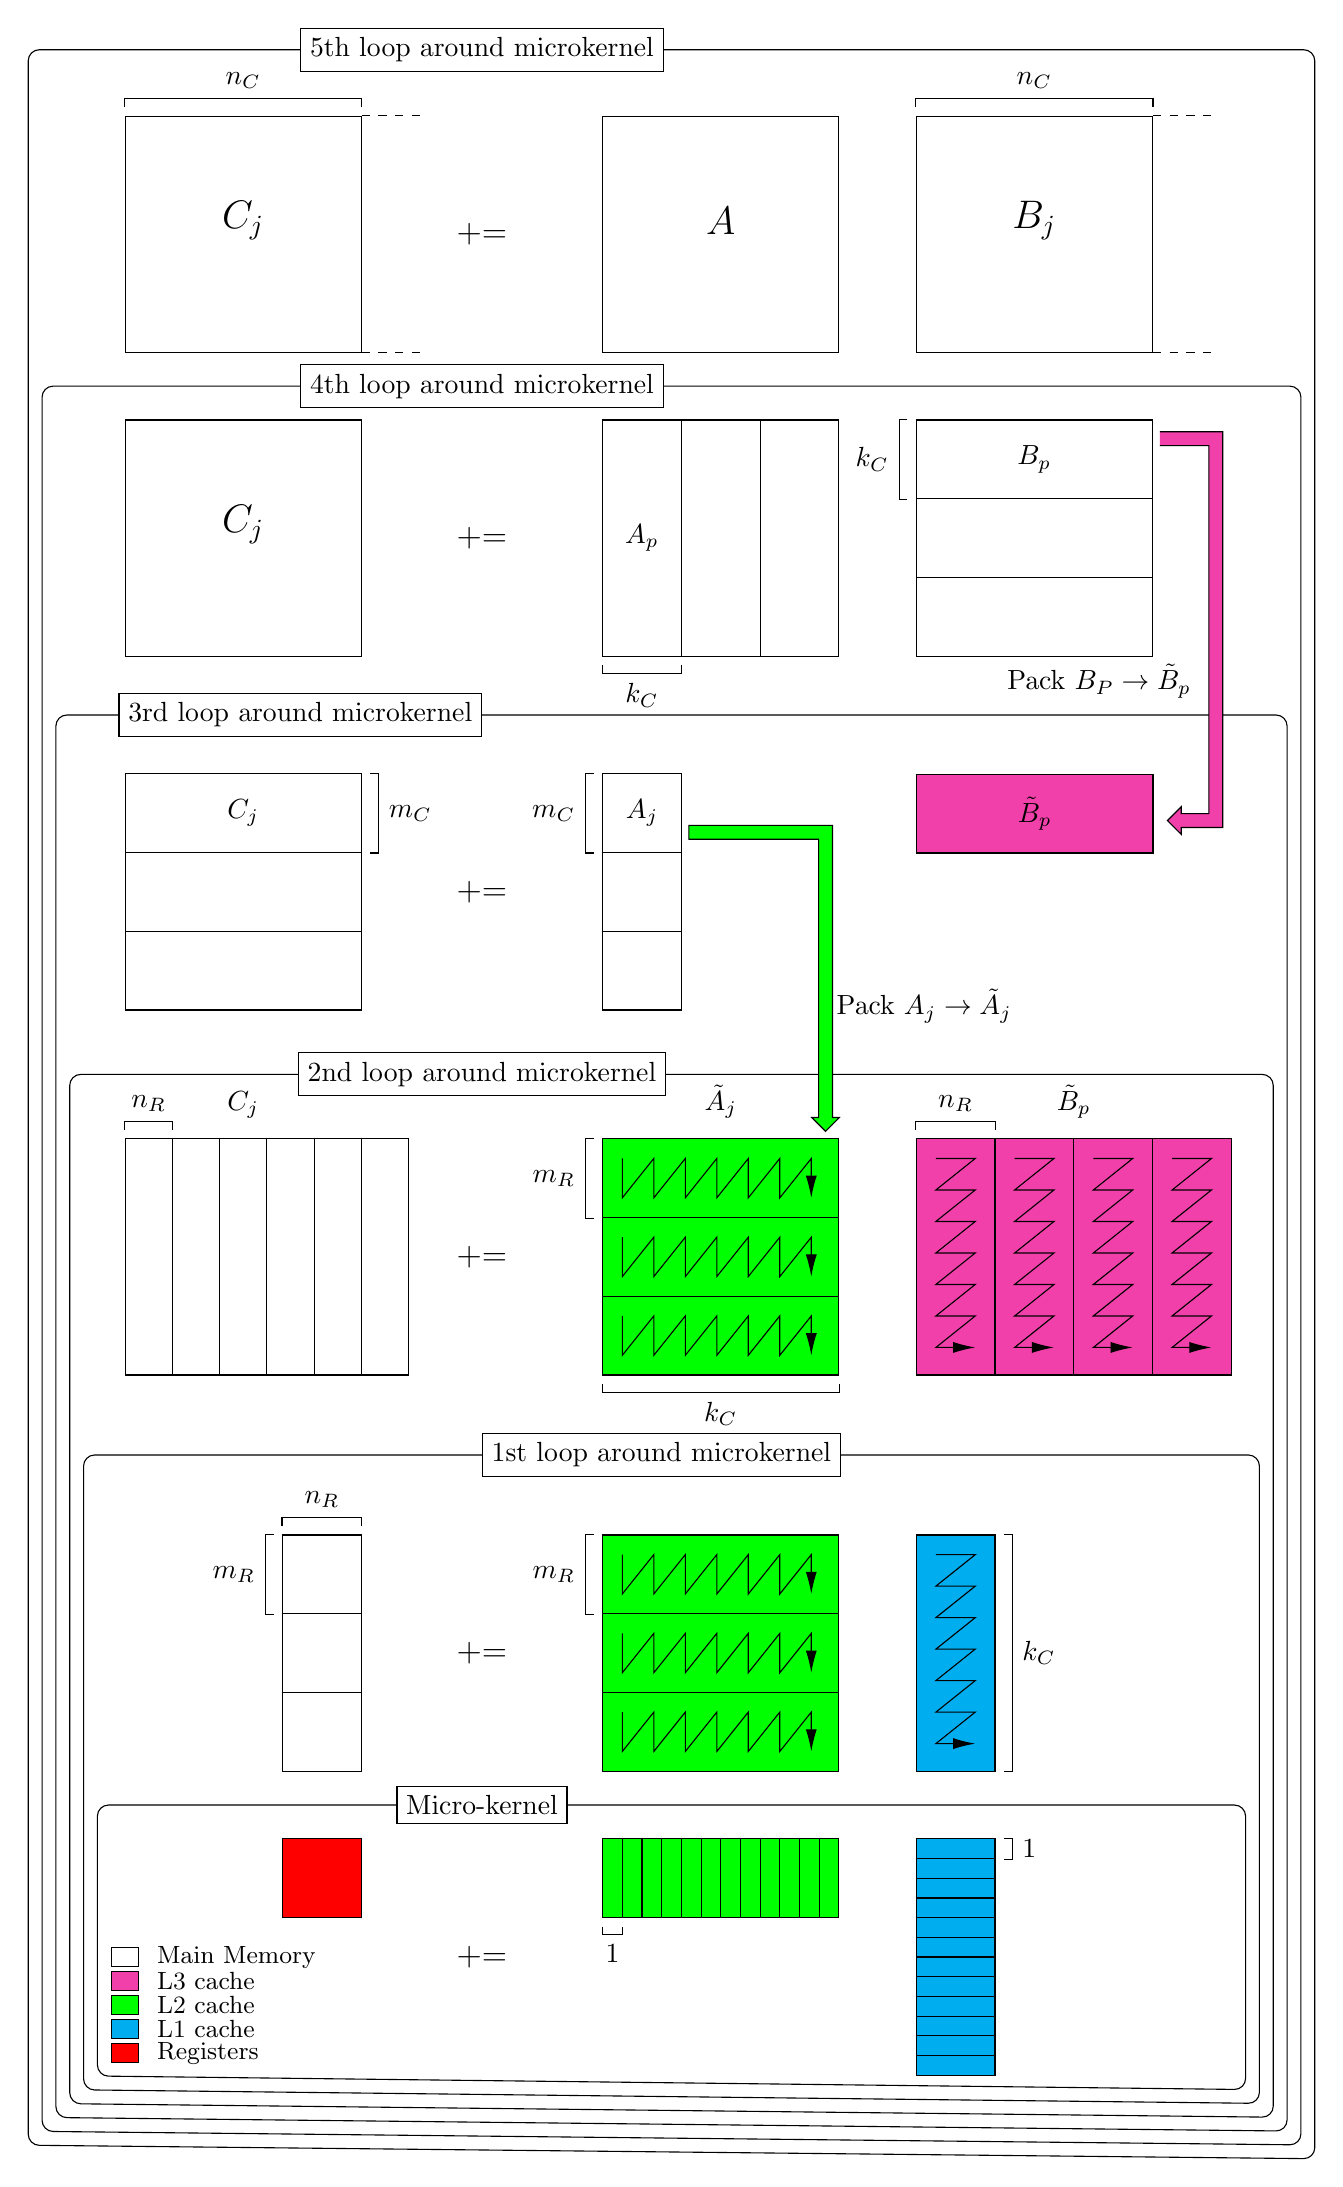
\begin{tikzpicture}
\matrix (loops)[column sep=0.2cm, row sep=5.5ex] {
  \node[square-mat] (5C) {\Large $C_j$};
  \bracelabel{5C.north west}{5C.north east}{above}{$n_C$}
  \draw[dashed] (5C.north east) -- ++(0.75, 0)
  (5C.south east) -- ++(0.75, 0);&

  \pluseqnode{5}&

  \node[square-mat,memory] (5A) {\Large $A$};&

  \node[square-mat,memory] (5B) {\Large $B_j$};
  \bracelabel{5B.north west}{5B.north east}{above}{$n_C$}
  \draw[dashed] (5B.north east) -- ++(0.75, 0)
  (5B.south east) -- ++(0.75, 0);\\


  \node[square-mat,memory] (4C) {\Large $C_j$};&

  \pluseqnode{4}&

  \vgrids[memory]{4A}{1}{3}{3}{}
  \node[at=(4A1)] {$A_p$};
  \bracelabel{4A1.south west}{4A1.south east}{below}{$k_C$}&

  \hgrids[memory]{4B}{3}{1}{3}{}
  \node[at=(4B1)] {$B_p$};
  \bracelabel{4B1.north west}{4B1.south west}{left}{$k_C$}\\


  \hgrids[memory]{3C}{3}{1}{3}{}
  \node[at=(3C1)] {$C_j$};
  \bracelabel{3C1.north east}{3C1.south east}{right}{$m_C$}&

  \pluseqnode{3}&

  \hgrids[memory]{3A}{1}{1}{3}{}
  \node[at=(3A1)] {$A_j$};
  \bracelabel{3A1.north west}{3A1.south west}{left}{$m_C$}&

  \node[rectangle,draw,l3,at={(0, 0)},anchor=north west, minimum height=1cm, minimum width=3cm] (3B) {$\tilde{B}_p$};\\


  \vgrids[memory]{2C}{0.6}{3}{6}{}
  \bracelabel{3C1.north west}{2C1.north east}{above}{$n_R$}
  \path (2C1.north west) -- (2C5.north east) node[midway,label={above:$C_j$}] {};&

  \pluseqnode{2}&

  \hgrids[l2]{2A}{3}{1}{3}{\apackarr{\y}}
  \bracelabel{2A1.north west}{2A1.south west}{left}{$m_R$}
  \bracelabel{2A3.south west}{2A3.south east}{below}{$k_C$}
  \path (2A1.north west) -- (2A1.north east) node[midway,label={above:$\tilde{A}_j$}] {};&

  \vgrids[l3]{2B}{1}{3}{4}{\bpackarr{\x}}
  \bracelabel{2B1.north west}{2B1.north east}{above}{$n_R$}
  \path (2B1.north west) -- (2B4.north east) node[midway, label={above:$\tilde{B}_p$}] {};\\


  \foreach \y in {1,...,3} {
    \node[rectangle, draw, fit={(2, -\y + 1) (3, -\y)}, inner sep=0] (1C\y) {};
  }
  \bracelabel{1C1.north west}{1C1.south west}{left}{$m_R$}
  \bracelabel{1C1.north west}{1C1.north east}{above}{$n_R$}&

  \pluseqnode{1}&

  \hgrids[l2]{1A}{3}{1}{3}{\apackarr{\y}}
  \bracelabel{1A1.north west}{1A1.south west}{left}{$m_R$}&

  \vgrids[l1]{1B}{1}{3}{1}{\bpackarr{\x}}
  \bracelabel{1B1.north east}{1B1.south east}{right}{$k_C$}\\


  \node[rectangle, draw, regs, fit={(2, 0) (3, -1)}, inner sep=0] (0C) {};
  \begin{scoped}[start chain=labels going {below=2pt of \tikzchainprevious}]
    \node[legend=Main Memory, memory] at (0, -1.5) {};
    \node[legend=L3 cache, l3] {};
    \node[legend=L2 cache, l2] {};
    \node[legend=L1 cache, l1] {};
    \node[legend=Registers, regs] {};
  \end{scoped}&

  \pluseqnode{0}&

  \vgrids[l2]{0A}{0.25}{1}{12}{}
  \bracelabel{0A1.south west}{0A1.south east}{below}{$1$}&

  \hgrids[l1]{0B}{1}{0.25}{12}{}
  \bracelabel{0B1.north east}{0B1.south east}{right}{$1$}\\
};
\path node[draw,above=1.8cm of 5-plus] (5-loop){5th loop around microkernel}
(5-plus) -- (4-plus) node[loop-label] (4-loop){4th loop around microkernel}
(4-plus) -- (3-plus) node[loop-label,anchor=east] (3-loop) {3rd loop around microkernel}
(3-plus) -- (2-plus) node[loop-label] (2-loop) {2nd loop around microkernel}
(2-plus) -- (1-plus) node[loop-label,anchor=west] (1-loop) {1st loop around microkernel}
(1-plus) -- (0-plus) node[loop-label] (0-loop) {Micro-kernel};

\draw[rounded corners] let \p1 = ($(0B12.south east) + (18pt, -5pt)$),
\p2 = ($(2B4.south east) + (5pt, -5pt)$),
\p{east} = (\x2, \y1) in
(0-loop.west) -| ($(labels-end.south west) + (-5pt, -5pt)$) coordinate (0-rect-west)
-- (\p{east}) coordinate (0-rect-east)
|- (0-loop.east);

\loopborder{1}{0}
\loopborder{2}{1}
\loopborder{3}{2}
\loopborder{4}{3}
\loopborder{5}{4}

\path[draw, l2] (3A1.south east) ++(2.5pt, 5pt) coordinate (A-arr-start)
-| ($(2A1.north east) + (-7.5pt, 7.5pt)$) node[pos=0.8,right=3pt] {Pack $A_j \to \tilde{A}_j$}
-- ++(-2.5pt, 0) -- ++(5pt, -5pt) -- ++(5pt, 5pt) -- ++(-2.5pt, 0)
|- ($(A-arr-start) + (0pt, 5pt)$) -- cycle;

\path[draw, l3] (4B1.east) ++(2.5pt, 5pt) coordinate (B-arr-start)
-| ($(3B.east) + (20pt, 0pt)$) node[pos=0.82,left=3pt] {Pack $B_P \to \tilde{B}_p$} coordinate (B-arr-down)
-- ++ (-10pt, 0)
-- ++(0pt, 2.5pt) -- ++(-5pt, -5pt) -- ++(5pt, -5pt) -- ++(0, 2.5pt)
-- ($(B-arr-down) + (5pt, -5pt)$)
|- ($(B-arr-start) + (0pt, 5pt)$);
\end{tikzpicture}
\end{document}
